\section{Experiments}
\label{sec:experiments}
%% =====================================================================

\subsection{Protocol}
\label{sec:protocol}

\textbf{Network, routing, and instances.}
The lower-level network, the time-window router, and the independent checker are fixed. The extended experiment matrix uses \textbf{five instances}:
the small instance \texttt{example\_3x3x2}, the congested instance \texttt{congested\_8x4x4},
and three \texttt{S8x4x4} layouts, \texttt{high}, \texttt{funnel}, and \texttt{mid}.
The last three share the same size and flexibility and differ only in corridor topology, so differences in impact-set size among them can be attributed to topology rather than to problem size.
The five instances come from two sources. The first two are hand-crafted layouts (the small instance allows step-by-step checking; the congested instance has a dumbbell topology). The last three are produced by our instance
generator; its parameters (number of jobs \(\times\) number of machines \(\times\) number of AGVs, congestion level, heterogeneity \(h\), and flexibility \(f\))
are encoded in the instance file name together with the \textbf{generation seed}, which is \(42\) for all three.
\textbf{The generation seed is independent of the run seeds used below}: the former determines only the instance itself, whereas the latter determine the disturbance injection
and the search process. Both sets of values contain \(42\), but no seed is shared between them.
\textbf{We use ten run seeds}, namely \(42\), \(7\), \(2024\), \(99\), \(123\), \(13\), \(1\),
\(777\), \(31415\), and \(8\), giving \(\NInst\times\NSeeds=\NPairs\) instance--seed pairs; each pair is called a ``cell'' below.
All cell-wise comparisons, win/loss counts, and paired tests in this paper are aligned on the key (instance, random seed):
under the same key, all methods read the same initial solution, the same blockage, and the same decision time.
The initial schedule is obtained by replaying the time-window router of Section~\ref{sec:reservation} in processing order,
and it passes the independent conflict-free check; all baseline methods share this initial solution within the same instance--seed pair.
We require only that \(\mathcal{S}^0\) be feasible before the disturbance.

\textbf{Implementation and computing environment.}
All experiments are implemented in pure Python with the standard library only, without third-party numerical libraries; the lower-level network, the time-window router, and the independent checker
reuse the same implementation as our static integrated work. Everything runs on a single machine in a single thread, without parallelism: Intel Xeon W-1270
(\(8\) cores, \(16\) threads), \(64\)\,GB RAM, Windows 10, and the CPython \(3.7.6\) interpreter (\(64\)-bit).
Because no third-party numerical library is used, reproduction requires no pinned dependency versions; \(3.7\) is the interpreter we tested,
and newer versions have not been rerun one by one. All timing results were obtained under the single-machine, single-thread setting above.
Different hardware would shift them uniformly, so all our runtime conclusions are stated as \emph{ratios} or \emph{orders of magnitude} and do not rely on absolute milliseconds.

\textbf{Code and data availability.}
The reproduction materials consist of three parts: the upper-level bounded repair and experiment drivers; the lower-level network and time-window router;
and the instances, disturbance inputs, and all cell-wise results (CSV). All three, together with the scripts that generate every table and figure, are submitted
and are available during review as an \textbf{anonymous repository} (see the link attached in the submission system; the repository contains no author-identifying information).
Upon acceptance, the repository will be made public and registered with a DOI in a permanent archiving service; this section will then be updated with that DOI.
Every table and figure can be traced in the repository to the script that generates it and to the corresponding CSV,
and the instances listed in Table~\ref{tab:instscale} are distributed with the repository.

\textbf{Second batch: externalizing the layout source.}
All five instances above use layouts designed by us, and the three same-size layouts also belong to one dumbbell family (they differ only in the number of parallel lanes at the load/unload station
exit and in the middle section, that is, only in capacity, not in geometry). To ensure that the layouts are not chosen by us, we run an additional batch of
\NPubInst\ instances. Three items of the network---the grid size, the placement of the load/unload station and the machines, and the missing edges---are transcribed item by item from the layout figures in
Appendix~A of Lyu et al.~\cite{lyu2019approach}, and the transcription is reconciled field by field by a script against the machine-readable encoding
provided with the van Os toolkit. The number of machines is therefore determined by the layout rather than chosen by us, and ranges from \(4\) to \(8\).
The same ten random seeds are used, giving \NPubPairs\ instance--seed pairs in total. The two batches are \emph{matched parameter by parameter}: the number of jobs,
the number of AGVs, the number of operations per job, \(h\), \(f\), and the calibration target of the transport-to-processing time ratio are all identical, so the difference between the two batches
can be attributed solely to the layout source.

That appendix gives six layouts in total (\(3\) to \(8\) machines). We do not use the \(3\)-machine layout: with \(f=0.6\) fixed and \(|M|=3\),
the average number of candidate machines is \(1.8<2\), which is incompatible with the requirement that ``every operation has at least two candidate machines''; relaxing \(f\) for a single layout
would introduce an extra variable.

The remaining five layouts \textbf{fall on only \NPubNets\ distinct networks}: the \(4\)-machine and \(5\)-machine layouts share
the same \(4\times 4\) grid (with the same edge removed), and the \(6\)-, \(7\)-, and \(8\)-machine layouts share the same
\(5\times 5\) grid (with the same two edges removed). The five differ from one another in the number of machines and their \emph{placement},
not in network geometry (this is how the original published data are organized). Therefore, when Section~\ref{sec:e4} analyzes this batch,
\textbf{the number of independent samples along the network-geometry dimension is \NPubNets, not \NPubInst}, whereas along the machine-placement dimension
it is \NPubInst; all claims below are stated according to this division.

This batch differs from the original data in three respects. \textbf{First, the per-edge travel times are not original data.} Lyu published per-edge durations only for a single example
instance, and those values are not uniform; the per-edge durations of the Appendix~A layouts were never published. We therefore fill them in
with ``all edges equally weighted,'' which is structurally consistent with the assumption of a ``constant unit-step duration'' in the van Os model and differs only in the scale of
the time unit. Consequently, the results of this batch are not compared with the reference values of Lyu or van Os; the batch serves only as a set of topologies not designed by us. \textbf{Second, the load and unload stations are merged.} The original layouts have separate
loading and unloading stations, whereas our setting has a single load/unload station; we therefore take the loading station at the vehicles' starting location as the load/unload station and treat the unloading station as an ordinary
grid node. \textbf{Third, their job data are not used.} In the public instance families we have measured, the average transport time is only a few percent of the average
processing time, so transport hardly causes any contention; if their job data were also adopted, corridor contention and all
phenomena that depend on it would become unobservable. Hence only the network is externalized.
Another family of layouts shipped with the same toolkit (labeled Liu 2023 in its directory) is not included in this batch: these layouts allow diagonal
moves, whereas our corridors are 4-connected; supporting diagonal moves would require modifying the lower-level router, not just the instances.

\textbf{Disturbances.}
Unless otherwise noted, \(t_{\mathrm{now}}=0.35\,C_{\max}(\mathcal{S}^0)\).
E1--E3 and E5 impose a single-window blockage on a busy corridor; E6 adds three further disturbance types at the same \(t_{\mathrm{now}}\);
E4 blocks the corridors in the LU cut (Section~\ref{sec:e4});
the disturbance-magnitude sweep sorts future operations by their earliest future reservation and takes the reservation windows of the first fraction \(\varphi\) as micro-blockages (without merging them).

\textbf{Baseline methods.}
R1: scoping on the affected set of the operation-precedence graph + level-1 rerouting, with \(\theta=2\) throughout
(this value affects only the size of \(|U_{R1}|\) under Class A disturbances; by Proposition~\ref{prop:miss}, any finite \(\theta\) yields an empty set under
Class B). Its scoping rule is taken from the operation-level
local rescheduling approach described in Section~\ref{sec:rw_aor} and is reimplemented by us. The correspondence is as follows. The scoping rule ``take the directly disturbed operations as the affected set,
then expand forward along the within-job operation precedence'' corresponds to
AOR~\cite{abumaizar1997rescheduling,subramaniam2003maor}.
The two further components, \emph{truncating the expansion at \(\theta\) hops} and \emph{mapping the operation set to the corridor reservations to be released},
are specified by us---the original setting has no reservation table, so this mapping has no counterpart there.
The rerouting and replay components share the same implementation as R2, so that the two differ only in the scope object.
R1 is therefore a baseline that transplants this scoping rule into our reservation setting; its results reflect how the rule performs in this setting,
not how the original method performs in its own setting.
R2/\STRC: scoping on the reservation impact set + level-1 rerouting (scope escalation after failure is enabled in the magnitude sweep and disabled in E3/E5).
R0+: global rescheduling that searches again within a time limit, starting from the original schedule---a genetic algorithm with population size \(40\),
the chromosome of the original schedule seeded into the initial population, and the same fixed-prefix decoding as RD (occupancies before \(t_{\mathrm{now}}\)
are not rewritable). \emph{No generation limit or early-stopping threshold is set}; the only termination condition is the wall-clock budget,
whose values are given in Section~\ref{sec:e5}.
RS: global right shift, which neither scopes on the impact set nor reroutes (Section~\ref{sec:cheap}).
RD: re-decoding of the original chromosome, the cheapest global recomputation in our implementation (same section).
RA: no restriction to the impact set but rerouting retained, that is, all unfinished occupancies after \(t_{\mathrm{now}}\) are made rewritable; everything else is identical to R2,
so that the role of the reservation impact set is tested in isolation (same section).
These five baselines are organized along ``whether the scope is delineated \(\times\) the recomputation range'': R1 and R2 differ only in the scope \emph{object};
RA and R2 differ only in \emph{whether} the scope is delineated (the rerouting procedure is identical); RS neither delineates the scope nor reroutes but pushes everything back;
RD and R0+ recompute globally without scoping on the impact set and differ only in how many generations they search.

\textbf{Budget convention.}
The methods are not compared at the same budget level. R1, R2, RS, RD, and RA are each a single deterministic repair
that terminates when the run finishes; their runtime is determined by instance size and impact-set size rather than by a budget setting. Only R0+ terminates on a wall-clock budget.
All results involving R0+ are therefore results under a given budget; the four-method comparison in Section~\ref{sec:cheap} is the one made within the same budget level
(each method runs once and terminates). Wall-clock times are reported per batch and are not compared across batches.

\textbf{Switch for scope escalation after failure.}
Scope escalation after failure is disabled in E3. If it were enabled, R1 might restore feasibility after escalating to all unfinished occupancies,
and the measurement would capture the fallback capability of the escalation rule rather than the difference between scope objects. Escalation is effective in itself (in the magnitude sweep it restores feasibility in all
cells), but it is unrelated to the variable under test, so it is disabled in the boundary ablation.
Its end point is exactly RA in Section~\ref{sec:cheap}, where it is measured cell by cell as an independent baseline, including its cost.

\textbf{Division of labor between the two batches.}
The two batches are not two samples of the same body of evidence; they answer different questions.
The main batch answers \emph{whether the phenomena exist and whether the mechanism can be identified in isolation}: under Class B disturbances, scoping on the operation-precedence graph yields an empty scope while the original schedule is infeasible
(Section~\ref{sec:e1}); the reservation impact set contains that scope and the fields outside the set remain invariant (Section~\ref{sec:e2});
and only the scope object is replaced under the same rerouting procedure (Section~\ref{sec:e3}). All three require full control over the instance parameters,
especially the transport-to-processing time ratio that determines whether corridor contention arises, and the public instance families cannot provide such control
(Section~\ref{sec:limitations}, limitation 4). The second batch answers a different question: \emph{whether these phenomena
hold only on layouts we chose ourselves}. It is used mainly for reproduction (Section~\ref{sec:pubrepro})
and yields no new performance-comparison conclusions.

The two batches are analyzed jointly in only two places. The first is E4. The three same-size layouts of the main batch belong to one family with very small geometric differences,
so two explanations---``the indicator is too coarse'' and ``the instances differ too little in geometry''---cannot be distinguished. Conversely, without a self-built baseline matched parameter by parameter,
the external layouts alone could not tell whether the variation in their impact-set share is large enough. The second batch accordingly narrows the conclusion on structural predictability.
The second is E5: the E5 protocol and parameters are identical in both batches, and pooling serves only to increase the number of cells without changing the direction of the conclusions.
The conclusions of all other sections are drawn from the main batch alone; the second batch only strengthens their external validity.

\textbf{Statistical convention.}
The paper contains two inferential tests, both in Section~\ref{sec:cheap}: the difference between R2 and RA in rewrite fraction (the primary test)
and the difference between R2 and RD in makespan. Both use the two-sided Wilcoxon signed-rank test, paired on the (instance, random seed) key defined above.
After Holm correction for these two tests, the significance conclusion of each is unchanged. All other cell-wise win/loss counts, means, and medians
are \emph{descriptive} statistics, and no significance claims are made for them.
The effect size accompanying the primary test is reported as a Hodges--Lehmann estimate of \(0.037\), with a \(95\%\) bootstrap confidence interval of
\([0.018,\,0.074]\) (percentile method, \(10^4\) resamples, fixed random seed); the mean paired difference is
\(\RAStabMean\), with interval \([0.039,\,0.093]\). Dispersion is reported as the interquartile range: the rewrite fraction has an IQR of
\(0.073\) for R2 and \(0.062\) for RA.
% selfcheck:allow-num 0.073 is the IQR of the R2 rewrite fraction; it equals \RAStabMeanNet (mean reduction after excluding identical cells) in value but comes from a different source
Because the two methods tie exactly in \(18\) of the \(50\) cells, the lower end of the confidence interval for the \emph{median} paired difference is \(0\);
this shows that ties make up about one third of the win/tie/loss counts.
The tables of all other batches give only means, medians, and counts, without intervals.

\subsection{E1: the operation-precedence graph yields an empty scope}
\label{sec:e1}

This section examines only what scope each of the two scoping rules yields under Class B disturbances; it does not compare repair quality.
Table~\ref{tab:e1} and Figure~\ref{fig:e1e3} (left) summarize the extended results for Proposition~\ref{prop:miss} under the corridor-blockage protocol of Section~\ref{sec:protocol}:
in \(\PassMiss\) cells, \(T_{\mathrm{impact}}=0\), the seed set and the reservation impact set are nonempty, and the original schedule is infeasible after the blockage.

Table~\ref{tab:e1} merges the three conditions into the column ``All three hold'' (cell-wise results are in the
\texttt{n\_T\_impact} and \texttt{feasible\_after\_block} columns of \texttt{e1\_miss.csv}).
Here \(T_{\mathrm{impact}}=0\) follows directly from the convention of Definition~\ref{def:task_impact} for Class B;
the substantive result is that the latter column is always false, that is, the original schedule \emph{is} indeed infeasible. Together, the two constitute a counterexample.

\begin{table}[t]
\centering
\caption{E1: the operation-precedence graph yields an empty scope under corridor blockage (\(\NSeeds\) random seeds per instance, \(\NPairs\) pairs in total).
\(|R|\) is the number of occupancies in the whole table, and \(\mathrm{Cl}/|R|\) is the share of the reservation impact set in the whole table. Means are taken over random seeds.
Dispersion is reported as the interquartile range (IQR): the per-instance IQR of \(\mathrm{Cl}/|R|\) lies
between \EoneFracIqrLo\ and \EoneFracIqrHi; over the \(\NPairs\) pooled pairs, the median is \EoneFracMed\ and
the range is \EoneFracMin--\EoneFracMax. The between-instance variation of this share is thus of the same order as its between-seed variation,
and the means should not be read in isolation.
``All three hold'' is the number of cells in which the three conditions of Proposition~\ref{prop:miss} hold simultaneously (\(T_{\mathrm{impact}}=0\),
a nonempty seed set, and an infeasible original schedule after the blockage). The last three rows share the same size and flexibility and differ only in corridor topology.}
\label{tab:e1}
\small
\begin{tabular}{@{}lcccccc@{}}
\toprule
Instance & Seeds & \makecell{All three\\hold} & Mean \(|R|\) & Mean \(|\mathrm{Src}|\)
 & Mean \(|\mathrm{Cl}|\) & \(\mathrm{Cl}/|R|\) \\
\midrule
\texttt{example\_3x3x2}   & 10 & \(10/10\) & \(28.6\)  & \(5.6\)  & \(16.9\) & \(0.59\) \\
\texttt{congested\_8x4x4} & 10 & \(10/10\) & \(85.0\)  & \(15.0\) & \(48.4\) & \(0.57\) \\
\texttt{S8x4x4} (high)    & 10 & \(10/10\) & \(150.5\) & \(15.5\) & \(88.3\) & \(0.59\) \\
\texttt{S8x4x4} (funnel)  & 10 & \(10/10\) & \(149.1\) & \(15.5\) & \(85.4\) & \(0.57\) \\
\texttt{S8x4x4} (mid)     & 10 & \(10/10\) & \(147.6\) & \(15.0\) & \(82.8\) & \(0.56\) \\
\midrule
Total & \(\NPairs\) & \(\PassMiss\) & --- & --- & --- & --- \\
\bottomrule
\end{tabular}
\end{table}

The absolute value of \(|\mathrm{Cl}|\) grows with the instance (\(16.9\), \(48.4\), \(82.8\)--\(88.3\)), a direct consequence of the larger total number of occupancies.
By contrast, \(\mathrm{Cl}/|R|\) lies within \EoneCloLo--\EoneCloHi\ on all five instances and \emph{fails} to distinguish the three \(\texttt{S8x4x4}\) layouts.
This agrees with the conclusion of Section~\ref{sec:e4}: the experiments yield no structural indicator that reliably predicts the impact-set size.
In terms of contributions, this section supports C1: under Class B disturbances, scoping on the operation-precedence graph yields an empty scope although the original schedule is already infeasible.

\subsection{E2: containment}
\label{sec:e2}

Structural closure (E2a) holds in \(\PassClosed\) cells (leakage \(=0\)), consistent with Proposition~\ref{prop:struct}.
Level-1 repair (without scope escalation) is feasible in \(\NPairs/\NPairs\) cells.
The corridor, time interval, and vehicle of every occupancy outside the set remain unchanged (E2b, the observable form of Proposition~\ref{prop:outside}), which likewise holds in \(\PassInvar\) cells
(Table~\ref{tab:e2}).

\begin{table}[t]
\centering
\caption{E2: containment (\(\NSeeds\) random seeds per instance; the level-1 feasibility column uses no scope escalation).
E2a is structural closure (leakage \(=0\));
E2b is the invariance of the corridor, time interval, and vehicle of \emph{every} occupancy outside the set.}
\label{tab:e2}
\small
\begin{tabular}{@{}lccc@{}}
\toprule
Instance & E2a closed & Level-1 feasible & \makecell{E2b outside set\\invariant per occupancy} \\
\midrule
\texttt{example\_3x3x2}   & \(10/10\) & \(10/10\) & \(10/10\) \\
\texttt{congested\_8x4x4} & \(10/10\) & \(10/10\) & \(10/10\) \\
\texttt{S8x4x4} (high)    & \(10/10\) & \(10/10\) & \(10/10\) \\
\texttt{S8x4x4} (funnel)  & \(10/10\) & \(10/10\) & \(10/10\) \\
\texttt{S8x4x4} (mid)     & \(10/10\) & \(10/10\) & \(10/10\) \\
\midrule
Total & \(\PassClosed\) & \(\NPairs/\NPairs\) & \(\PassInvar\) \\
\bottomrule
\end{tabular}
\end{table}

E2a and E2b mean different things. E2a is a property \emph{of the graph}, guaranteed by Proposition~\ref{prop:struct},
and serves to check that the implementation agrees with the definition. E2b is a property \emph{after repair}; it tests whether the four premises of Proposition~\ref{prop:outside}
hold under our protocol. Premise (ii) requires that every occupancy outside the set be pre-committed successfully; if an occupancy outside the set overlaps a no-entry window,
the pre-commit fails, which indicates that the seed set is incomplete (Remark~\ref{rem:precommit}).
In terms of contributions, E1, E2, and the boundary ablation in Section~\ref{sec:e3} support the \emph{object level} of C1 and C2: the reservation impact set
is uniquely determined by the edge set, is closed under outgoing edges, and restores feasibility in every cell under the same rerouting procedure. The net benefit of scoping is given by
the RA baseline in Section~\ref{sec:cheap}.

\begin{remark}[An implementation defect misread as an edge-set defect]
\label{rem:e2b_history}
If rerouting is decided per \emph{operation} rather than per \emph{occupancy}, E2b passes in only \(24/\NPairs\) cells,
which is easily misread as ``the dependency edge set fails to cover some weak couplings.'' The actual cause is a granularity mismatch: the rewritable set consists of \emph{occupancies},
whereas under per-operation decisions the whole transport is replanned as soon as either its empty leg or its loaded leg falls in the impact set.
When only the loaded leg enters the impact set, the empty leg of the same operation is also rewritten, even though its task label is not in the rewritable set;
it is therefore recorded as drift outside the set. All \(84\) drifting occupancies in the \(26\) failing cells are such same-operation empty legs,
and \(71\) of them (\(85\%\)) had already been executed before \(t_{\mathrm{now}}\), so rewriting them also violates Assumption A2.
After switching to per-\emph{leg} decisions (empty legs that have been executed or are not made rewritable keep their original plan,
and only legs in the rewritable set are rerouted), the drift drops to zero.
Hence what was measured was not how well the edge set covers the physical couplings, but the fact that premise (iii) of Proposition~\ref{prop:outside},
``the router is invoked only for transports in \(U\),'' was not satisfied by the implementation.
The general form of this misjudgment is to misread a granularity mismatch between implementation and definition as a lack of expressiveness in the model.

\textbf{A mismatch of the same kind that E2b cannot detect.} Under per-leg decisions, a leg that \emph{spans}
\(t_{\mathrm{now}}\) is still replanned as a whole: as soon as one of its segments ends later than
\(t_{\mathrm{now}}\), the task label of the entire leg enters the rewritable set, so the segments it had \emph{already traversed} before
\(t_{\mathrm{now}}\) are rescheduled as well. This amounts to sending the vehicle back to the start of the leg to drive it again, which violates Assumption A2.
E2b cannot detect this case, because the task labels of these segments lie \emph{inside} the impact set and are thus outside the scope of the comparison of fields outside the set.
The case is detected by a separate audit of finished occupancies (comparing, one by one, the occupancies with \(t^e\le t_{\mathrm{now}}\)):
\(36\) of the \(\NPairs\) cells contain such rewrites, \(86\) in total.
After refining the granularity to \emph{segments} (segments already traversed are kept as they are, and rerouting starts from the node where the vehicle actually is at
\(t_{\mathrm{now}}\)), the audit drops to zero in all \(\NPairs\) cells,
all pass rates are unchanged, and \(C_{\max}\) improves in \(6\) cells and worsens in none.
All tables in this paper report results of the segment-granularity implementation; the numbers in this remark (\(24/\NPairs\); \(84\) occupancies in \(26\) cells; \(86\) occupancies in \(36\) cells)
all come from the coarser-granularity implementations.
\end{remark}

\subsection{E3: boundary ablation}
\label{sec:e3}

Table~\ref{tab:e3} and Figure~\ref{fig:e1e3} (right) fix level-1 rerouting and \emph{disable} scope escalation after failure.
Under Class B disturbances, R1 has an empty rewritable set and is infeasible in \(\NPairs/\NPairs\) cells, whereas R2 is feasible in all cells.

The two arms use the same rerouting procedure, the same initial solution, the same \(t_{\mathrm{now}}\), the same random seeds, and the same blockage window;
\textbf{the only difference is which occupancies are rewritable}. R1's rewritable set is empty, and level-1 rerouting is the identity operation on an empty set,
so the original schedule is left unchanged and still occupies the blocked corridor. R1 therefore fails because it decides that no rescheduling is needed, not because of repair quality.
The cell-wise runtime of level-1 rerouting has a median of \(\MsRepairMed\)\,ms and a maximum of \(\MsRepairMax\)\,ms; the last column of Table~\ref{tab:e3}
is the mean over the \(\NSeeds\) random seeds within each instance. The two statistics are defined differently and are not directly comparable.
In terms of contributions, this section attributes the gap to the scope object (C2, C3): with the same rerouting procedure and only the scope object replaced, the feasibility rate changes from
\(\FeasRone\) to \(\FeasRtwo\).

We separately test whether this contrast depends on the calibration of edge weights. Our corridor edges are equally weighted, so we rerun E1 and E3 on the same \(\NPairs\) pairs
under three non-uniform edge-weight settings
(\texttt{lognormal}, \texttt{lu\_far}, and \texttt{split}; data in \texttt{weight\_sweep.csv}). The results for ``all three hold'' and for the empty operation-precedence-graph scope are unchanged at every setting;
R1 remains infeasible in all cells, and the numbers of level-1-feasible cells for R2 are \WeightLogRtwo, \WeightLuRtwo, and \WeightSplitRtwo, respectively.
The only infeasible cell occurs under the \texttt{split} setting (\texttt{S8x4x4\_high}, random seed \(1\)).
The contrast therefore does not depend on the equal-weight calibration.

\begin{table}[t]
\centering
\caption{E3: boundary ablation (no scope escalation; \(\NInst\) instances \(\times\) \(\NSeeds\) random seeds).
miss\_B means that in the cell, R1's rewritable set is empty whereas R2's is nonempty.
The last column is the mean over the \(\NSeeds\) random seeds within each instance, which differs from the cell-wise median reported in the text.}
\label{tab:e3}
\small
\begin{tabular}{@{}lccccc@{}}
\toprule
Instance & miss\_B & R1 feasible & R2 feasible & Mean \(|U_{R2}|\) & \makecell{R2 runtime\\/ms} \\
\midrule
\texttt{example\_3x3x2}   & \(10/10\) & \(0/10\) & \(10/10\) & \(16.9\) & \(0.66\) \\
\texttt{congested\_8x4x4} & \(10/10\) & \(0/10\) & \(10/10\) & \(48.4\) & \(2.84\) \\
\texttt{S8x4x4} (high)    & \(10/10\) & \(0/10\) & \(10/10\) & \(88.3\) & \(3.40\) \\
\texttt{S8x4x4} (funnel)  & \(10/10\) & \(0/10\) & \(10/10\) & \(85.4\) & \(5.09\) \\
\texttt{S8x4x4} (mid)     & \(10/10\) & \(0/10\) & \(10/10\) & \(82.8\) & \(3.96\) \\
\midrule
Total & \(\NPairs/\NPairs\) & \(\FeasRone\) & \(\FeasRtwo\) & --- & --- \\
\bottomrule
\end{tabular}
\end{table}

\begin{figure}[t]
\centering
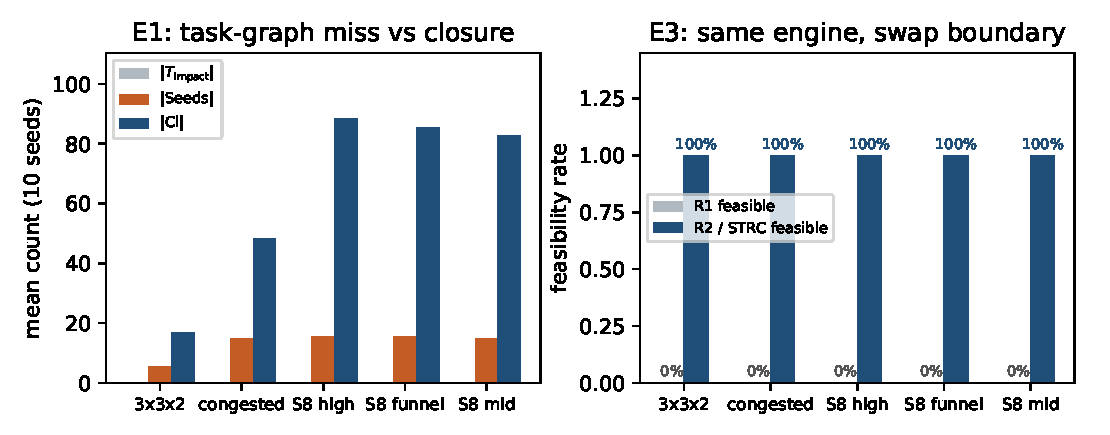
\includegraphics[width=\linewidth]{figures/fig_strc_e1e3}
\caption{Visualization of the extended E1/E3 results (means over \(\NInst\) instances \(\times\) \(\NSeeds\) random seeds).
Left: the affected set on the operation-precedence graph is empty, whereas the seed set and the reservation impact set are nonempty. Bar heights are means over the \(\NSeeds\) cells
of each instance; dispersion as IQR is given in Table~\ref{tab:e1} (the per-instance IQR of \(|\mathrm{Cl}|\) lies between \(2\) and \(8\);
the affected-set group is always zero and thus has no dispersion).
Right: with the same rerouting and only the scope object replaced, the feasibility rate is \(0\) for R1 and \(100\%\) for R2; this panel shows cell-wise counts
(\(\NPairs\) cells each), so no dispersion is given.}
\Description{Two bar charts side by side. The left panel shows, for each of the five instances, three groups of bars: the affected set on the operation-precedence graph, the number of seed occupancies, and the size of the reservation impact set.
The affected-set group is always zero, and the other two grow with instance size. The right panel shows the feasibility rate
of the two scoping rules: zero for scoping on the operation-precedence graph and one hundred percent for scoping on the reservation impact set.}
\label{fig:e1e3}
\end{figure}

\subsection{Case Gantt chart}
\label{sec:case}

\begin{sloppypar}
E1--E3 report counts and feasibility rates across random seeds. To show on the operation timeline a case that ``the operation-precedence graph cannot capture but scoping on the reservation impact set can repair,''
Figure~\ref{fig:case} takes one corridor blockage on \texttt{example\_3x3x2} with random seed \(42\).
The protocol is the same as in E2/E3: the decision time is \(0.35\,C_{\max}\), a busy corridor is blocked in a single window, and level-1 rerouting is used without scope escalation.
\end{sloppypar}

In this case \(T_{\mathrm{impact}}=\varnothing\), whereas \(|\mathrm{Src}|=6\) and \(|\mathrm{Cl}|=18\).
Figure~\ref{fig:case}(a) is the machine Gantt chart of the original schedule before the disturbance: blue operations have transport occupancies in the impact set (to be rerouted),
and gray operations lie outside the impact set (pre-committed and kept as planned); the red dashed line marks \(t_{\mathrm{now}}\), and the light red band marks the blockage window.
Figure~\ref{fig:case}(b) shows the schedule after repair: the operations in the impact set are rearranged on the timeline, and the schedule regains feasibility under the blockage, with
\(C_{\max}:57\to 86\) and a sub-millisecond runtime.
This figure only illustrates what kind of local change the statistical conclusions correspond to; it is not used to compare makespans.
The trade-off in makespan against global rescheduling is examined in E5 and in the disturbance-magnitude sweep.

\begin{figure}[t]
\centering
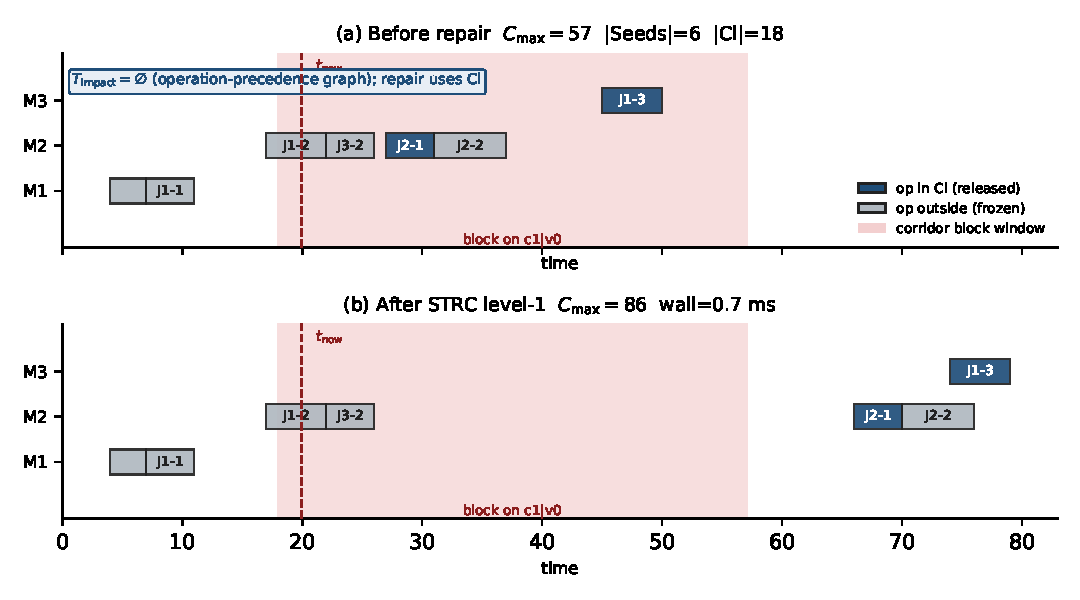
\includegraphics[width=\linewidth]{figures/fig_strc_case}
\caption{Case Gantt chart (\texttt{example\_3x3x2}, random seed \(42\)).
(a)~Original schedule before the blockage, colored by membership in \(\mathrm{Cl}\);
(b)~after level-1 repair. The affected set on the operation-precedence graph is empty; blue operations are those whose transports in the impact set are rerouted.
The figure only illustrates the form of the local change.}
\Description{Two machine Gantt charts stacked vertically. (a) The original schedule before the blockage; bars are colored blue or gray according to whether their transport occupancies fall in
the reservation impact set, a vertical red dashed line marks the decision time, and a light red vertical band marks the blockage window.
(b) The repaired schedule; the blue bars are rearranged on the timeline, the gray bars stay in place, and the makespan increases from 57 to 86.}
\label{fig:case}
\end{figure}

